\documentclass[11pt,a4paper]{article}
\usepackage[T1]{fontenc}
\usepackage[margin=2.3cm]{geometry}
\usepackage{amsmath,amssymb}
\usepackage{graphicx}
\usepackage[dvipsnames]{xcolor}
\usepackage{enumitem}
\usepackage[colorlinks=true,linkcolor=blue,urlcolor=blue]{hyperref}
\setlength{\parskip}{0.6em}
\setlength{\parindent}{0pt}
\begin{document}

\begin{center}{\LARGE\bfseries openbeam}\\[0.4em]{\large Find the lightest beam that does not sag too much, in three sessions.}\\[0.2em]\small PAN IIT OSS explainer \textbullet{} diploma / undergraduate to advanced undergraduate (levels 5-6)\end{center}

\section*{Why this exists}
Every floor, shelf and bridge deck rests on beams. This explainer shows the mathematics of a loaded beam: how the load is shared between the supports, how the inside forces vary along the beam, and how much the beam bends. It uses only simple formulas and a small numerical solver, so you can build it yourself.

\section*{The end goal}
Meet a deflection limit with the lightest beam (shear, moment, deflection). The end goal is to meet a deflection limit with the lightest beam. That is the heart of structural design: choose a shape and a depth so that the beam is stiff enough and strong enough using as little material as possible. These are classroom models of straight elastic beams and never replace the checks of a qualified engineer.

\section*{How the three sessions build up}
\begin{enumerate}[nosep]
\item \textbf{Session 1: Reactions, shear and moment: what a beam does with a load} (Level 1, conceptual interactive model, 60 min).
\item \textbf{Session 2: Stiffness and strength: second moment of area, deflection and stress} (Level 2, mathematical engineering model, 80 min).
\item \textbf{Session 3: Solve it numerically: a finite-element beam, validated and refined} (Level 3, simulation and validation, 90 min).
\end{enumerate}

\section{Session 1: Reactions, shear and moment: what a beam does with a load}

\subsection*{A. Real-world problem}
A plank across a stream bends when you stand on it. Two things hold it up: the two banks. How much of your weight does each bank carry? Where inside the plank is the bending worst? Engineers answer with three pictures: the reactions at the supports, the shear force diagram and the bending moment diagram. This repo is a classroom model: it teaches the ideas, and is never a tool for designing a real structure.

\subsection*{B. Concept and theory}
A simply supported beam of span L rests on a support at x = 0 (A) and x = L (B). A downward point load P acts at distance a from A, and b = L - a from B. The beam stays still, so forces balance (RA + RB = P) and turning effects about A balance (RB L = P a). Cutting the beam at x and keeping the left piece shows what the inside of the beam must supply: a vertical shear force V and a bending moment M. M is largest where V changes sign. The slope of the moment diagram equals the shear force.

\begin{itemize}[nosep]
\item P: point load (downward) (kN)
\item L: span between supports (m)
\item a, b: distances of the load from support A and B (b = L - a) (m)
\item RA, RB: support reactions (upward) (kN)
\item V(x): shear force at position x (kN)
\item M(x): bending moment at position x (sagging positive) (kN m)
\end{itemize}

\begin{equation*}
R_A=\frac{P\,b}{L},\qquad R_B=\frac{P\,a}{L},\qquad R_A+R_B=P
\end{equation*}

\begin{equation*}
V(x)=R_A\ (x<a),\qquad V(x)=R_A-P\ (x>a)
\end{equation*}

\begin{equation*}
M(x)=R_A\,x\ (x\le a),\qquad M(x)=R_A\,x-P\,(x-a)\ (x\ge a),\qquad M_{\max}=\frac{P\,a\,b}{L}
\end{equation*}

\begin{center}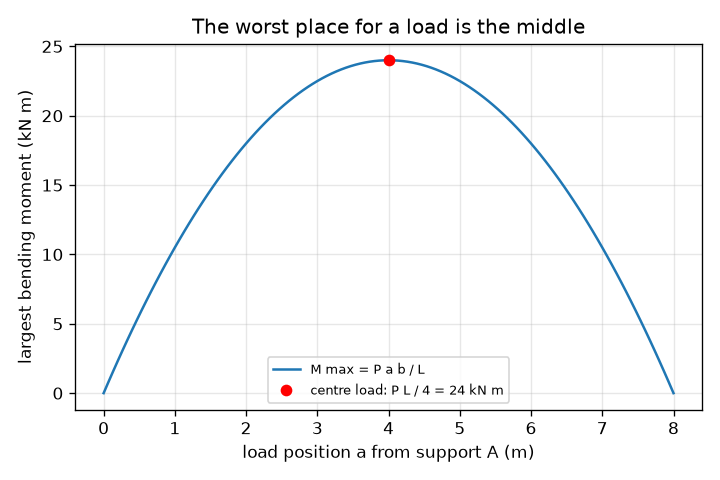
\includegraphics[width=0.85\linewidth]{figures/s01_moment_vs_position.png}\\\small The largest moment against load position: highest at the centre, P L / 4 = 24 kN m.\end{center}

\subsection*{E. Worked example}
A beam spans L = 8 m. A load P = 12 kN acts at a = 2 m from the left support. Find the reactions, the shear force on each side of the load and the largest bending moment.
\begin{enumerate}[nosep]
\item b = L - a = 8 - 2 = 6 m.
\item Turning about A: RB x 8 = 12 x 2, so RB = 24 / 8 = 3 kN.
\item Forces: RA = 12 - 3 = 9 kN. Check with RA = P b / L = 12 x 6 / 8 = 9 kN.
\item Shear: V = +9 kN from x = 0 to 2 m, then 9 - 12 = -3 kN from 2 m to 8 m.
\item Largest moment is under the load: M = RA x a = 9 x 2 = 18 kN m. Check from the right: RB x b = 3 x 6 = 18 kN m. The two agree and equal P a b / L = 12 x 2 x 6 / 8 = 18 kN m.
\end{enumerate}
\textbf{Answer.} RA = 9 kN, RB = 3 kN; shear +9 kN then -3 kN; largest moment 18 kN m at x = 2 m.

\subsection*{F. Questions}
\begin{enumerate}[nosep]
\item \textbf{Conceptual.} Why does the support closer to the load carry more of it? What happens to the two reactions when the load slides to exactly the middle?
\item \textbf{Numerical.} A 20 kN load acts 1.5 m from the left support of a 5 m beam. Find RA, RB and the largest bending moment, with units, and check that the answers are sensible.
\item \textbf{Graph and simulation interpretation.} On the moment graph, where is the peak, what is the slope of the line to its left, and what does that slope equal on the shear graph?
\item \textbf{Design and optimisation challenge.} A shelf plank can take at most 15 kN m of bending moment. The load is 10 kN on a 6 m span. In which positions along the span may the load stand, if any?
\end{enumerate}

\section{Session 2: Stiffness and strength: second moment of area, deflection and stress}

\subsection*{A. Real-world problem}
Two planks of the same wood and width span a stream. One lies flat, the other stands on edge. The one on edge hardly bends. Why, when both hold the same amount of wood? And if a rule says the beam may sag at most L/360 and the wood may not be stressed beyond a limit, what is the lightest beam that passes? (Classroom model, not a design method: real design codes add load factors, material grades and many more checks.)

\subsection*{B. Concept and theory}
How much a beam bends depends on the loads and on its stiffness EI: the material stiffness E (Young's modulus) times the shape stiffness I (second moment of area). Material far from the neutral axis counts more, because each small area dA contributes y squared times dA, so depth enters as h cubed. For a point load the deflected curve and the maximum deflection follow from Euler-Bernoulli beam theory. The bending stress at distance y from the neutral axis is M y / I; it is largest at the top and bottom faces.

\begin{itemize}[nosep]
\item E: Young's modulus of the material (Pa (GPa in the app))
\item I: second moment of area of the cross-section (m\textasciicircum{}4 (mm\textasciicircum{}4))
\item b, h: width and depth of a rectangular section (m (mm))
\item v(x): downward deflection at position x (m (mm))
\item sigma: bending stress (Pa (MPa))
\item y: distance from the neutral axis (m)
\item L/360: common deflection limit (span divided by 360) (m)
\end{itemize}

\begin{equation*}
I_{\mathrm{rect}}=\frac{b\,h^{3}}{12},\qquad I_{\mathrm{I}}=\frac{b_f h^{3}-(b_f-t_w)(h-2t_f)^{3}}{12}
\end{equation*}

\begin{equation*}
v(x)=\frac{P\,b\,x\,(L^{2}-b^{2}-x^{2})}{6\,E\,I\,L}\ (x\le a),\qquad v_{\max}=\frac{P\,L^{3}}{48\,E\,I}\ \text{(load at centre)}
\end{equation*}

\begin{equation*}
\sigma=\frac{M\,y}{I},\qquad \sigma_{\max}=\frac{M_{\max}\,(h/2)}{I},\qquad M_{\max}=\frac{P\,a\,b}{L}
\end{equation*}

\begin{center}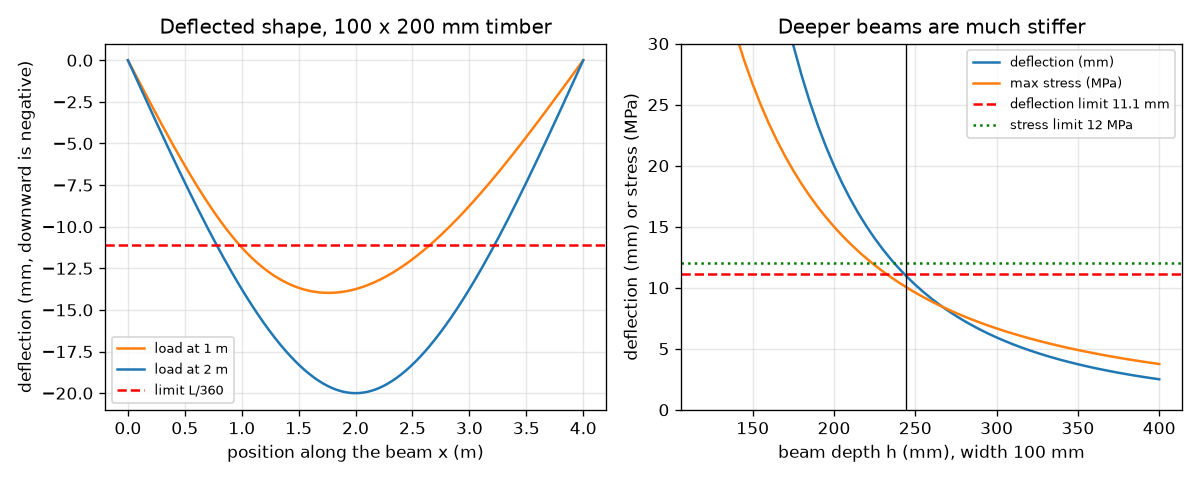
\includegraphics[width=0.85\linewidth]{figures/s02_deflection_design.png}\\\small Left: deflected shape against the L/360 limit. Right: deflection and stress against beam depth; the vertical line marks the lightest passing depth, 244 mm.\end{center}

\subsection*{E. Worked example}
A timber beam (E = 10 GPa) spans L = 4 m with a 10 kN load at mid-span. The section is 100 mm wide and 200 mm deep. Find I, the maximum deflection, the maximum stress, and compare with L/360 and 12 MPa.
\begin{enumerate}[nosep]
\item I = b h\textasciicircum{}3 / 12 = 0.100 x 0.200\textasciicircum{}3 / 12 = 6.667 x 10\textasciicircum{}-5 m\textasciicircum{}4 (66.67 x 10\textasciicircum{}6 mm\textasciicircum{}4).
\item Deflection = P L\textasciicircum{}3 / (48 E I) = 10 000 x 64 / (48 x 10 x 10\textasciicircum{}9 x 6.667 x 10\textasciicircum{}-5) = 640 000 / 32 000 000 = 0.0200 m = 20.0 mm.
\item Limit L/360 = 4 / 360 = 11.1 mm. The beam sags too much.
\item M max = P L / 4 = 10 x 4 / 4 = 10 kN m. Stress = M (h/2) / I = 10 000 x 0.100 / 6.667 x 10\textasciicircum{}-5 = 15.0 MPa. This is above 12 MPa too.
\item Fix by depth: deflection scales as 1/h\textasciicircum{}3, so we need h \textgreater{}= 200 x (20 / 11.11)\textasciicircum{}(1/3) = 243.2 mm; stress scales as 1/h\textasciicircum{}2, so h \textgreater{}= 200 x sqrt(15/12) = 223.6 mm. Deflection governs. The lightest depth in whole millimetres is 244 mm (area 24 400 mm\textasciicircum{}2), with deflection 11.01 mm and stress 10.1 MPa.
\end{enumerate}
\textbf{Answer.} I = 6.667e-5 m\textasciicircum{}4, deflection 20.0 mm (too much), stress 15.0 MPa (too much); the lightest passing 100 mm wide rectangle is 244 mm deep.

\subsection*{F. Questions}
\begin{enumerate}[nosep]
\item \textbf{Conceptual.} Why does increasing a beam's depth often improve bending stiffness more effectively than adding the same amount of material near the neutral axis?
\item \textbf{Numerical.} A timber beam 50 mm wide and 150 mm deep, E = 12 GPa, spans 3 m with a 5 kN load at mid-span. Find the maximum deflection and stress, with units, and compare with L/360 and 12 MPa.
\item \textbf{Graph and simulation interpretation.} On the demand graph (demand divided by limit against depth) the blue curve crosses 1 at about 243 mm and the green curve at about 224 mm. Which limit governs and what does it mean for the designer?
\item \textbf{Design and optimisation challenge.} Design: with E = 10 GPa, L = 4 m and the 10 kN centre load, compare two ways of reaching the required stiffness: keep the width at 100 mm and increase the depth, or keep the depth at 200 mm and increase the width. Which uses less material, and by how much?
\end{enumerate}

\section{Session 3: Solve it numerically: a finite-element beam, validated and refined}

\subsection*{A. Real-world problem}
Real beams have distributed loads, several point loads and sections that change along their length. Formulas exist for only a few simple cases. A finite-element program cuts the beam into short elements and solves them together, but how do we know it is right? We run it on cases with exact answers, study what happens as the mesh is refined, and only then trust it on cases with no formula. And a simple question remains for the engineer: which is the lightest beam that sags less than L/360 and keeps its factor of safety? This is a classroom model; it is never a design tool for real structures.

\subsection*{B. Concept and theory}
The beam is cut into n elements of length le. Each node has a deflection w and a slope theta. Inside an element the deflection is a cubic (Hermite) curve, which is the exact solution of the beam equation between loads, so a 4 x 4 stiffness matrix links the four end values to the four end forces. The element matrices are added into a global matrix K, loads are turned into a force vector F, the supports remove some unknowns, and solving K d = F gives all w and theta. The bending moment follows from the curvature, M = -EI w''; here it is averaged over each element, so it converges more slowly than the deflection. Euler-Bernoulli theory ignores shear deformation, which adds about E h\textasciicircum{}2 / (kappa G L\textasciicircum{}2) of extra deflection to a centre-loaded rectangular beam.

\begin{itemize}[nosep]
\item n: number of elements (none)
\item le: element length L / n (m)
\item w, theta: nodal deflection (downward) and slope (m, rad)
\item K, F, d: global stiffness matrix, load vector, unknowns (N/m, N and N m, m and rad)
\item q: uniform load per metre (N/m)
\item EI: bending stiffness (N m\textasciicircum{}2)
\item fos: factor of safety on yield: yield stress / actual stress (none)
\item kappa: shear coefficient of the section (5/6 for a rectangle) (none)
\end{itemize}

\begin{equation*}
k_e=\frac{EI}{l_e^{3}}\begin{pmatrix}12&6l_e&-12&6l_e\\6l_e&4l_e^{2}&-6l_e&2l_e^{2}\\-12&-6l_e&12&-6l_e\\6l_e&2l_e^{2}&-6l_e&4l_e^{2}\end{pmatrix},\qquad K\,d=F
\end{equation*}

\begin{equation*}
w_{\mathrm{centre}}=\frac{P\,L^{3}}{48\,EI},\qquad w_{\mathrm{UDL}}=\frac{5\,q\,L^{4}}{384\,EI},\qquad w_{\mathrm{tip}}=\frac{P\,L^{3}}{3\,EI}
\end{equation*}

\begin{equation*}
\frac{w_{\mathrm{shear}}}{w_{\mathrm{bend}}}\approx\frac{E\,h^{2}}{\kappa\,G\,L^{2}}=\frac{2(1+\nu)}{\kappa\,(L/h)^{2}}
\end{equation*}

\begin{center}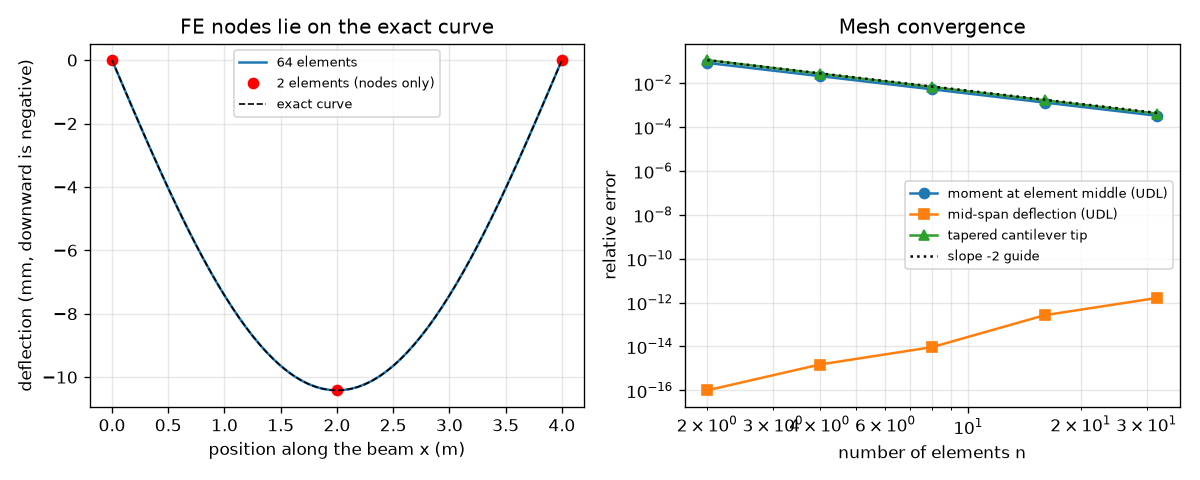
\includegraphics[width=0.85\linewidth]{figures/s03_fe_validation.png}\\\small Left: 2-element nodes (dots) lie on the exact curve. Right: log-log error against the number of elements for moment, deflection and a tapered beam.\end{center}

\subsection*{E. Worked example}
A simply supported steel beam spans L = 4 m with E I = 200 GPa x 8.0e-6 m\textasciicircum{}4 = 1.6e6 N m\textasciicircum{}2. Find the mid-span deflection (a) for a 10 kN centre load, (b) for a uniform load of 5 kN/m, and compare each with the finite-element solver on a 2-element and an 8-element mesh. Then give both loads together.
\begin{enumerate}[nosep]
\item (a) w = P L\textasciicircum{}3 / (48 E I) = 10 000 x 64 / (48 x 1.6e6) = 640 000 / 76 800 000 = 0.008333 m = 8.333 mm.
\item (b) w = 5 q L\textasciicircum{}4 / (384 E I) = 5 x 5000 x 256 / (384 x 1.6e6) = 6 400 000 / 614 400 000 = 0.010417 m = 10.417 mm.
\item Run solve\_beam: the 2-element mesh gives 8.3333 mm for (a), the 8-element mesh gives 10.4167 mm for (b). They agree with the formulas to 7 digits or better, because for constant EI the cubic element is exact at the nodes.
\item Both loads act together: deflections add (superposition for a linear elastic beam), 8.333 + 10.417 = 18.75 mm.
\item Why still refine the mesh? The moment is a second derivative of w; the element-average moments approach the true moment only as the elements shrink (error about 4 / (3 n\textasciicircum{}2) of the peak for a uniform load).
\end{enumerate}
\textbf{Answer.} 8.333 mm for the centre load, 10.417 mm for the uniform load, 18.75 mm for both; the solver matches to better than 1e-7.

\subsection*{F. Questions}
\begin{enumerate}[nosep]
\item \textbf{Conceptual.} The finite-element deflection is exact at the nodes even with 2 elements, but the bending moment is not. Why?
\item \textbf{Numerical.} A simply supported beam of span 5 m, EI = 2.0e6 N m\textasciicircum{}2 carries a uniform load of 4 kN/m. Find the mid-span deflection and its maximum moment with units, and say what the 4-element solver's moment error against the peak should be.
\item \textbf{Graph and simulation interpretation.} On the log-log convergence plot, the moment error is 2.1\% of the peak for n = 8. Estimate it for n = 32 and say what slope the line has.
\item \textbf{Design and optimisation challenge.} Design: for the footbridge girder (6 m span, 3.5 kN/m, 5 kN at mid-span, steel, flanges 150 x 10 mm, web 6 mm, depths in 10 mm steps) find the lightest passing depth with a factor of safety of 1.5, and then with a factor of safety of 3. Which limit governs and what does it cost in mass?
\end{enumerate}

\section{Real-world mini-project}
\textbf{Check a footbridge girder (classroom exercise only).} A small footbridge span of 6 m rests on two identical steel girders. One girder carries a uniform service load of 3.5 kN/m (deck and pedestrians) plus a 5 kN point load at mid-span, and its own weight. Steel: E = 200 GPa, yield stress 250 MPa. Required: deflection at most L/360 and a factor of safety of 1.5 on the yield stress. Try I-sections with flanges 150 mm x 10 mm and a web 6 mm thick, with depths from 100 mm to 400 mm in steps of 10 mm, using \texttt{check\_footbridge} from Session 3. This is a teaching exercise: real footbridges also need vibration, buckling, connection and load-combination checks by a qualified engineer, and nothing here may be used to design or assess a real structure.

\section{The path ahead}
\begin{enumerate}[nosep]
\item \textbf{Session 4: Lightest I-section by search.} A search over I-section dimensions for the footbridge girder, with the proportion limits you choose and state.
\item \textbf{Session 5: Moving-load envelope.} A function that sweeps a two-axle load (2 x 10 kN, 3 m apart) along a 12 m span and records the largest moment at each section.
\item \textbf{Session 6: Continuous beam with a middle support.} An extension of \texttt{solve\_beam} with an interior support, for two equal spans under a uniform load.
\item \textbf{Session 7: Shear deformation (Timoshenko element).} A beam element that includes shear deformation.
\item \textbf{Session 8: Depth-versus-weight explorer.} An animation or app that shows the beam, the shear, moment and deflection diagrams and the lightest passing depth for any span.
\end{enumerate}

\section{Answers and hints}

\subsection*{Session 1}
\begin{enumerate}[nosep]
\item \textbf{Conceptual.} Hint: Think of a see-saw: which end must push harder to stop it turning? Solution: Balance of turning effects about the far support shows that the near support must supply the bigger share (RA = P b / L is bigger when b, the distance to the far support, is bigger). At the middle a = b = L / 2, so both reactions equal P / 2.
\item \textbf{Numerical.} Hint: b = 3.5 m. Use RA = P b / L and M = RA a. Solution: RA = 20 x 3.5 / 5 = 14 kN, RB = 20 x 1.5 / 5 = 6 kN. Check: 14 + 6 = 20 kN. M max = 14 x 1.5 = 21 kN m (also 6 x 3.5 = 21 kN m). The bigger reaction is on the side nearer the load, as expected.
\item \textbf{Graph and simulation interpretation.} Hint: The slope of M against x is the shear force V. Solution: The peak is directly under the load. To its left M rises in a straight line whose slope is RA (in kN m per m, which is kN); that equals the positive shear step on the shear graph. To the right M falls with slope -RB, the negative shear step. The peak is where V changes sign.
\item \textbf{Design and optimisation challenge.} Hint: Solve P a (L - a) / L \textless{}= 15 for a, or compare with the centre value P L / 4. Solution: The centre is the worst case: P L / 4 = 10 x 6 / 4 = 15 kN m, exactly at the limit. So the plank passes everywhere (it is just at its limit in the middle). Trade-off: any extra load, or a longer span, would break the limit at the centre. Assumption: own weight is ignored.
\end{enumerate}

\subsection*{Session 2}
\begin{enumerate}[nosep]
\item \textbf{Conceptual.} Hint: Write I = b h\textasciicircum{}3 / 12 and ask what each small piece of area contributes, and how far from the axis it is. Solution: Each small piece of area contributes y squared times dA to I, so pieces far from the neutral axis count much more than pieces near it. Material put into depth is placed farther from the axis (and I grows as h cubed), while the same material added next to the axis, for example as extra width, only multiplies I by the same factor as the width (I grows only linearly with b). Example: adding 20\% area as depth multiplies I by 1.728, as width only by 1.2.
\item \textbf{Numerical.} Hint: I = b h\textasciicircum{}3 / 12; deflection = P L\textasciicircum{}3 / (48 E I); M = P L / 4. Solution: I = 0.050 x 0.150\textasciicircum{}3 / 12 = 1.406 x 10\textasciicircum{}-5 m\textasciicircum{}4. Deflection = 5000 x 27 / (48 x 12 x 10\textasciicircum{}9 x 1.406 x 10\textasciicircum{}-5) = 0.0167 m = 16.7 mm, against the limit 3000 / 360 = 8.33 mm: fails. M = 5 x 3 / 4 = 3.75 kN m; stress = 3750 x 0.075 / 1.406 x 10\textasciicircum{}-5 = 20.0 MPa, above 12 MPa: fails. Sanity check: a person-sized load on a slim plank sagging 17 mm over 3 m is believable.
\item \textbf{Graph and simulation interpretation.} Hint: The beam passes only when both curves are at or below 1. Solution: The beam needs a depth of at least the larger of the two crossing depths, 243 mm, so the deflection limit governs. The beam is then stronger than needed against stress (stress at 244 mm is about 10.1 MPa against 12 MPa). To lighten the beam the designer must increase stiffness per unit material, for example by choosing a shape with material far from the axis, or a stiffer material.
\item \textbf{Design and optimisation challenge.} Hint: Required I is 20 / 11.11 = 1.8 times the current I. Depth route: h\textasciicircum{}3 scales; width route: b scales. Solution: Required I = 1.8 x 6.667 x 10\textasciicircum{}7 = 1.2 x 10\textasciicircum{}8 mm\textasciicircum{}4. Depth route: h = 243.2 mm, area 100 x 243.2 = 24 320 mm\textasciicircum{}2. Width route: b = 100 x 1.8 = 180 mm, area 180 x 200 = 36 000 mm\textasciicircum{}2. The depth route uses about 32\% less material. Stress also passes both ways. Trade-offs: a deep thin beam may twist sideways (not modelled here) and may not fit the available room.
\end{enumerate}

\subsection*{Session 3}
\begin{enumerate}[nosep]
\item \textbf{Conceptual.} Hint: Between loads the exact deflection of a beam is a cubic curve. What does the moment need from the curve? Solution: The element's cubic shape functions can reproduce the exact deflection between loads, and the consistent load vector puts the nodal values on the exact curve (for constant EI). The moment needs the second derivative of w; the element-average second derivative approximates the true moment only to second order in the element length, so the moment converges as 1/n\textasciicircum{}2 instead of being exact.
\item \textbf{Numerical.} Hint: Use 5 q L\textasciicircum{}4 / (384 EI) and q L\textasciicircum{}2 / 8. The element-moment error against the peak is 4 / (3 n\textasciicircum{}2). Solution: w = 5 x 4000 x 625 / (384 x 2.0e6) = 12 500 000 / 768 000 000 = 0.01628 m = 16.3 mm. M max = 4000 x 25 / 8 = 12 500 N m = 12.5 kN m. For n = 4 the element-average error against the peak is 4 / (3 x 16) = 8.3\%, so the solver would show about 11.5 kN m. Sanity check: a 5 m steel beam sagging 16 mm (L/307) is plausible for a light section.
\item \textbf{Graph and simulation interpretation.} Hint: The line has slope -2: error proportional to 1/n\textasciicircum{}2. Solution: n = 32 is 4 times as many elements, so the error is 4\textasciicircum{}2 = 16 times smaller: 2.1\% / 16 = 0.13\% (the lesson prints 0.13\%). The slope is -2 on a log-log plot. Deflection errors, at round-off level, do not follow this line.
\item \textbf{Design and optimisation challenge.} Hint: Run check\_footbridge for each depth; the stress test is fos x stress \textless{}= 250 MPa; the deflection test is w \textless{}= L/360. Solution: With fos 1.5 the lightest passing depth is 190 mm: deflection 16.2 mm (limit 16.67 mm), stress 87.3 MPa, mass 31.6 kg/m. With fos 3, stress must be at most 83.3 MPa, which needs 200 mm (stress 82.1 MPa, mass 32.0 kg/m). The deflection limit governs with fos 1.5, and a doubled factor of safety costs only about 1.5\% in mass. Assumptions: static load only; real footbridges need vibration and buckling checks.
\end{enumerate}

\section{How to join}
Read \texttt{CONTRIBUTING.md} in the repository, then pick an issue labelled \texttt{good first issue}. Repository: \url{https://github.com/KrunalPanchal1995/openbeam}

\end{document}
